\documentclass[aps,prl,reprint,floatfix,superscriptaddress]{revtex4-1} %might want some options later
\usepackage{graphicx}
\usepackage{amsmath}
\usepackage{float}
\usepackage{hyperref}
\usepackage{epstopdf}

\begin{document}

\floatstyle{ruled}
\newfloat{program}{ht}{lop}
\floatname{program}{Example }

\title{Quantum Circuit Viewer}
\date{\today}
\author{Alex \surname{Parent}}
\email{aparent@uwaterloo.ca}
\author{Jacob \surname{Parker}}
\email{j3parker@uwaterloo.ca}
\author{Marc \surname{Burns}}
\email{m4burns@uwaterloo.ca}
\affiliation{Institute for Quantum Computing, University of Waterloo, Waterloo, ON, Canada}
\author{Dmitri \surname{Maslov}}
\email{dmaslov@iqc.ca}
\affiliation{Institute for Quantum Computing, University of Waterloo, Waterloo, ON, Canada}
\affiliation{National Science Foundation, Arlington, VA, USA}
\begin{abstract}
Quantum Circuit Viewer (QCViewer) is a software tool for the design and simulation of quantum circuits.  
It allows users to test new circuit designs and make publication quality diagrams with an easy to use graphical interface.  
Supported features also include simulation of the circuit while graphically displaying the current state.
It is also useful for viewing very large/complex circuits with the use of subcircuit abstraction.
\end{abstract}
\maketitle

\section{Introduction}
In creating QCViewer our goal was to develop a convenient tool that would be useful to the quantum computing community for both research and educational purposes. 
QCViewer provides a drag and drop interface for circuit design.  
This makes it easy to quickly test out new algorithm and circuit design ideas.
In order to make the diagrams useful for presentation and publication we provide the ability to export images in scalable vector graphics (\verb+.svg+), portable network graphics (\verb+.png+) and encapsulated postscript (\verb+.eps+) formats.

\section{Software}
The executable for QCViewer can be obtained from the website \url{http://qcirc.iqc.uwaterloo.ca/}.

\section{Circuit Format}
To store circuits we use our own circuit format which was somewhat inspired by the \verb+.tfc+ format used on the ``Reversible Logic Synthesis Benchmarks Page''\cite{maslovBench}. We use \verb+.qc+ as the extension for our circuit files, and all \verb+.tfc+ files are valid \verb+.qc+ files.
We will illustrate the construction of a circuit for Grover's algorithm.  
The representation we have chosen is taken from \cite{nielsen2000quantum}, page 256.
It can be found in the software distribution as \verb+demos/grover.qc+.
\subsection{Header}
A qubit name may be any ASCII text composed with letters and numbers. 
The \verb+.v+, \verb+.i+ and \verb+.o+ lists define qubit names, input qubits and output qubits respectively.
An optional \verb+.ol+ list allows alternate names for output labels.
See the header at the beginning of Example \ref{l:circuit}.

\subsection{Main Circuit}
The main circuit is specified between the \verb+BEGIN+ and \verb+END+ tags.
Each line contains a gate name followed by labels specifying which qubits the gate effects, with the first set of inputs being the controls and the last set of inputs of proper size being the target(s) of the gate.
An apostrophe after a qubit name indicates that the control is negative. 
For example, \verb+T a b' c+ specifies a Toffoli gate on qubit \verb+c+, positive control from qubit \verb+a+ and negative control from qubit \verb+b+. 

Single qubit rotations X, Y, and Z are supported using the R gate, for example \verb+RX(2 pi/3)+ would preform a rotation by $2\pi/3$ around the x-axis. 
Any gate defined in the user editable gate library is also supported.

When generating a diagram for a circuit, the gates are packed into columns in a greedy fashion. 
A semicolon at the end of a line will force a column break.

\subsection{Subcircuits}
A subcircuit can be specified between the \verb+BEGIN <name> (<arg> ..)+ and \verb+END <name>+ tags.
The arguments to a subcircuit are the names of the input qubits.
The scope of these arguments is exclusive to the subcircuit.
A subcircuit can then be included in the main circuit as if it were a gate.
We now build the complete \verb+.qc+ for Grover's algorithm using subcircuits and loops that are introduced in the next section.
Figure \ref{f:grover} is the diagram that QCViewer generates for the file content shown in Example \ref{l:circuit}.

\subsection{Loops}
Loops allow certain parts of the circuit to be executed multiple times. 
They are specified in the file format using the exponent symbol and subcircuits.
For example \verb+GroverIterate^4 a b c d e Workspace+ denotes that the subcircuit \verb+GroverIterate+ should be run four times.


\begin{figure*}[ht]
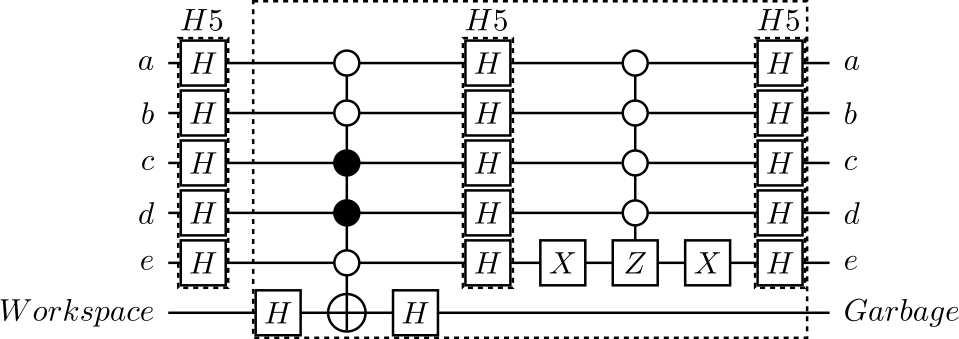
\includegraphics[scale=0.47]{grover_circuit}
\caption{Circuit diagram for Grover's algorithm example}
\label{f:grover}
\end{figure*}

\begin{program}
\begin{verbatim}
.v a b c d e Workspace
.i a b c d e Workspace
.o a b c d e

BEGIN 5H (a b c d e)
H a
H b
H c
H d 
H e
END 5H

BEGIN GroverIterate (a b c d e Workspace)
H Workspace
T a' b' c d e' Workspace
H Workspace
5H a b c d e
X e ; Z a' b' c' d' e ; X e
5H a b c d e
END GroverIterate

BEGIN
H5 a b c d e
GroverIterate^4 a b c d e Workspace
END
\end{verbatim}
\caption{Circuit file for Grover's algorithm.}
\label{l:circuit}
\end{program}
\subsection{Gates}\label{sub:gates}
Gates are specified in a gate library file to allow custom gate sets to be added easily.
For example, the specification of the Hadamard gate can be found in Example \ref{l:gate}.
\begin{program}
\begin{verbatim}
NAME Hadamard
SYMBOL H
1/sqrt(2) ,  1/sqrt(2)
1/sqrt(2) , -1/sqrt(2)
\end{verbatim}
\caption{Specification of the Hadamard gate.}
\label{l:gate}
\end{program}
\section{Circuit Design}
Circuits may be written directly in the specified file format as an ASCII file, or drawn graphically using a drag-and-drop interface.  
Gates can be placed by dragging them directly onto qubit wires.
Controls are then edited by entering control editing mode and clicking on qubit wires (two clicks to place a negative control).

\section{Circuit Simulation}
Our circuit simulator is state-vector based.
Breakpoints can be inserted into the circuit to pause the simulation at specific points.
The results of the simulation can be displayed as graphs of either the probability distribution, real amplitudes or imaginary amplitudes of the state in the computational basis.
\subsection{State Entry}
Input state may be specified using Dirac notation with states being automatically normalized if needed.
The input to the circuit implementing Grover's algorithm as illustrated in Figure \ref{f:grover} is \verb$|0>^5|1>$ or more simply \verb$|000001>$. 
More complex inputs are also supported, e.g., \verb$(|0>+|1>)^4 + 3/4|1011>$.


\bibliography{QCV}

\end{document}
